\section{Summary of Data}

The resulting forest was composed of 3007 instances, 1213 ideas, and 335 category trees. The number of instances, ideas and categories present in each of the number conditions is given in table TAG. In addition, table TAG shows the number of "non-singleton" categories, namely, those categories containing at least two instances. Intuitively, non-singleton categories represent those categories in which some exploration actually occured. These represent categories in which we can potentially identify the idea production phase of the SIAM model [].

\begin{tabular}[h!]{r | l l l l l l }
& 5 & 10 & 20 & 50 & 75 & 100 \\ \hline \hline
HITs & 57 & 47 & 23 & 10 & 10 & 10 \\
instances & 293 & 471 & 453 & 500 & 634 & 855 \\
ideas & 171 & 249 & 278 & 341 & 443 & 177 \\
category trees & 76 & 93 & 100 & 123 & 172 & 177 \\
non-singleton trees & 28 & 41 & 41 & 50 & 49 & 61 \\
\end{tabular}

Figure FIG shows the distribution of instances in non-singleton categories. The majority of the "mass" of instances are in trees with less than 70 instances.

% TODO: this figure needs better labeling for the second part
\begin{figure}[!h]
    \centering
    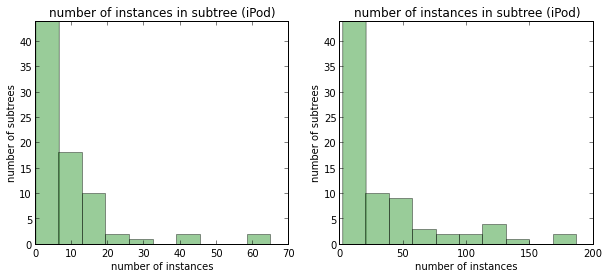
\includegraphics[width=0.9\columnwidth]{instances_in_subtrees}
\end{figure}